\documentclass[11pt,a4paper,english,reqno,a4paper]{amsart}
\usepackage{amsmath,amssymb,amsthm, graphicx}
\usepackage{tikz}

\begin{document}

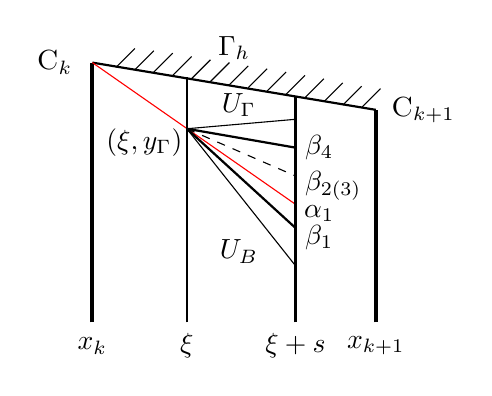
\begin{tikzpicture}[scale=0.6]
\draw [line width=0.05cm] (-3.5,-4.0) --(-3.5,1.5);
\draw [line width=0.05cm] (2.5,-4.0) --(2.5,0.5);
\draw [thick] (-3.5,1.5)--(2.5,0.5);

\draw [thin][red] (-3.5,1.5)--(0.8,-1.5);
\draw [line width=0.03cm] (-1.5,-4.0) --(-1.5,1.2);
\draw [line width=0.03cm] (0.8,-4.0) --(0.8,0.8);

\draw [thin](-1.5, 0.1) --(0.8,-2.8);
\draw [thick](-1.5, 0.1) --(0.8,-2.0);
\draw [dashed](-1.5, 0.1) --(0.8,-0.9);
\draw [thick](-1.5, 0.1) --(0.8,-0.3);
\draw [thin](-1.5, 0.1) --(0.8,0.3);

\draw [thin] (-3, 1.4) --(-2.6, 1.8);
\draw [thin] (-2.6, 1.35) --(-2.2, 1.75);
\draw [thin] (-2.2, 1.30) --(-1.8, 1.70);
\draw [thin] (-1.8, 1.23) --(-1.4, 1.63);
\draw [thin] (-1.4, 1.16) --(-1.0, 1.56);
\draw [thin] (-1.0, 1.10) --(-0.6, 1.50);
\draw [thin] (-0.6, 1.03) --(-0.2, 1.43);
\draw [thin] (-0.2, 0.97) --(0.2, 1.37);
\draw [thin] (0.2, 0.9) --(0.6, 1.30);
\draw [thin] (0.6, 0.83) --(1, 1.23);
\draw [thin] (1, 0.76) --(1.4, 1.16);
\draw [thin] (1.4, 0.67) --(1.8, 1.07);
\draw [thin] (1.8, 0.60) --(2.2, 1.0);
\draw [thin] (2.2, 0.55) --(2.6, 0.95);

\node at (1.3, -0.3){$\beta_{4}$};
\node at (1.6, -1.1){$\beta_{2(3)}$};
\node at (1.3, -1.7){$\alpha_{1}$};
\node at (1.3, -2.2){$\beta_{1}$};

\node at (-0.4, 0.6){$U_{\Gamma}$};
\node at (-0.4, -2.5){$U_{B}$};

\node at (-2.4, -0.2){$(\xi,y_{\Gamma})$};
\node at (-4.3, 1.5){$\textsc{C}_{k}$};
\node at (3.5, 0.5){$\textsc{C}_{k+1}$};
\node at (-0.5, 1.8){$\Gamma_h$};

\node at (-1.5, -4.5){$\xi$};
\node at (0.8, -4.5){$\xi+s$};
\node at (-3.5, -4.5){$x_{k}$};
\node at (2.5, -4.5){$x_{k+1}$};
\end{tikzpicture}

\end{document}